\documentclass[11pt,a4paper]{article}
\usepackage[utf8]{inputenc}
\usepackage[T1]{fontenc}
\usepackage{lmodern}
\usepackage[margin=2.5cm]{geometry}
\usepackage{booktabs}
\usepackage{graphicx}
\usepackage{enumitem}
\usepackage[hidelinks]{hyperref}

\newcommand{\todo}[1]{\textbf{[To fill in: #1]}}
\setlist{itemsep=2pt,topsep=4pt}

\title{Predicting Bug-Prone Files from Git History\\with Machine Learning}
\author{Your Name\\ \small Project 2: machine learning applied to a software engineering problem}
\date{November 2026}

\begin{document}
\maketitle

\begin{abstract}
\noindent Review and testing time is limited, so a team has to choose which
files to look at first. This project builds a model that reads the git history
of a project and gives every source file a risk score: how likely the file is
to need a bug fix in the following year. The data was collected for this
project from 12 open-source Python projects (129,357 commits, 2,492 source
files). Three classifiers were compared by always testing on a project that
was left out of training. The best one, logistic regression, reaches an
average AUC of 0.837 and an F1 score of 0.610 on unseen projects, and the 20\%
of files it ranks highest contain 48\% of the files that were later fixed.
A simple rule, ``largest files first'', is almost as good (AUC 0.827), which
shows that file size carries most of the signal.
\todo{one sentence on the user feedback from Section~\ref{sec:users}}
\end{abstract}

\section{Problem overview}

The software engineering activity addressed here is \emph{deciding where to
spend review and testing effort}. In most projects bugs are not spread evenly:
a small part of the files accounts for a large part of the
faults~\cite{ostrand}. If these files can be pointed out in advance, reviewers
can read them more carefully and testers can write tests for them first.

Developers usually make this choice from experience. That works for people who
have known the code for years, but not for new team members or for large
projects. The version control history contains the same knowledge in a form a
program can read: which files change often, how many people touch them, and
where bugs were fixed before. Earlier studies found that such history measures
predict defects well~\cite{nagappan,moser}.

The task is therefore: \emph{given the git history of a project up to today,
predict for every source file whether it will need a bug fix during the next
12 months.} This is a supervised binary classification problem with one row
per file.

\section{Data collection}

No existing dataset was used. The data was collected for this project directly
from public repositories on GitHub.

\paragraph{Projects.} Twelve well-known, actively maintained Python projects
from different areas were chosen (Table~\ref{tab:data}): machine learning,
data analysis, testing, web scraping, task queues, databases, type checking,
documentation, graphs, packaging, data validation and scientific arrays.

\paragraph{Collection.} For every project the script \texttt{collect\_data.py}
\begin{enumerate}
\item downloads the complete history with \texttt{git clone -{}-bare};
\item reads every commit with \texttt{git log -{}-numstat}: date, author,
      message, and for each changed file the number of lines added and
      deleted. Merge commits are skipped because they only join branches;
\item marks a commit as a \emph{bug fix} when the first line of its message
      contains one of the words \emph{fix, fixes, fixed, bug, bugfix, crash,
      regression} and none of \emph{typo, doc, docstring, comment}.
\end{enumerate}
In total 129,357 commits were read.

\paragraph{Time split.} A cutoff date in the past, 1~November 2025, separates
what the model may see from what it has to predict. Features are computed only
from commits before the cutoff. The label comes only from commits in the
12~months after it (until 1~November 2026). This copies the real situation:
the prediction is made on a given day, and the truth is known a year later.

\paragraph{Features.} Each file that existed at the cutoff is described by the
nine numbers in Table~\ref{tab:features}.

\begin{table}[h]
\centering
\begin{tabular}{ll}
\toprule
Feature & Meaning (all measured before the cutoff) \\
\midrule
\texttt{loc} & lines in the file at the cutoff \\
\texttt{commits} & number of commits that changed the file \\
\texttt{authors} & number of different people who changed it \\
\texttt{churn} & lines added plus lines deleted, over all commits \\
\texttt{bugfixes} & number of bug-fix commits that changed the file \\
\texttt{age\_days} & days since the file was created \\
\texttt{days\_since\_change} & days since the last change \\
\texttt{recent\_commits} & commits in the last 365 days \\
\texttt{recent\_bugfixes} & bug-fix commits in the last 365 days \\
\bottomrule
\end{tabular}
\caption{The features of a file.}
\label{tab:features}
\end{table}

\paragraph{Label.} A file is labelled \emph{buggy} (1) if at least one bug-fix
commit changed it in the 12 months after the cutoff, and \emph{clean} (0)
otherwise.

\paragraph{Filtering.} Only Python source files are kept. Files in test,
documentation, example and benchmark folders are removed, because a ``fix'' in
a test or in the documentation is not a defect of the product. Files for which
no history was found are removed as well.

\paragraph{Result.} The dataset has 2,492 files, of which 761 (30.5\%) are
buggy. Table~\ref{tab:data} shows that the projects differ a lot: the share of
buggy files goes from 8.7\% to 57.1\%.

\begin{table}[h]
\centering
\begin{tabular}{lrrr}
\toprule
Project & Files & Buggy & Share buggy \\
\midrule
celery/celery & 180 & 71 & 39.4\% \\
networkx/networkx & 289 & 35 & 12.1\% \\
pandas-dev/pandas & 301 & 172 & 57.1\% \\
pydantic/pydantic & 107 & 26 & 24.3\% \\
pydata/xarray & 111 & 53 & 47.7\% \\
pytest-dev/pytest & 81 & 37 & 45.7\% \\
python-poetry/poetry & 171 & 53 & 31.0\% \\
python/mypy & 297 & 107 & 36.0\% \\
scikit-learn/scikit-learn & 331 & 93 & 28.1\% \\
scrapy/scrapy & 169 & 51 & 30.2\% \\
sphinx-doc/sphinx & 229 & 20 & 8.7\% \\
sqlalchemy/sqlalchemy & 226 & 43 & 19.0\% \\
\midrule
Total & 2,492 & 761 & 30.5\% \\
\bottomrule
\end{tabular}
\caption{The dataset.}
\label{tab:data}
\end{table}

\section{Machine learning approach}

\paragraph{Type of learning.} The labels are known from history, so this is
supervised learning, and the answer is yes or no, so it is binary
classification. Each model also outputs a risk between 0 and 1, which is used
to rank the files.

\paragraph{Models.} Three standard classifiers for tables of numbers were
compared:
\begin{itemize}
\item \textbf{Logistic regression}: gives every feature a weight and turns the
      weighted sum into a risk. Simple and easy to interpret.
\item \textbf{Decision tree} (depth at most 5): a sequence of yes/no questions
      about the features.
\item \textbf{Random forest} (300 trees): many trees that vote. It can
      capture combinations of features that a single weight cannot.
\end{itemize}
Deep learning was not considered: the dataset has a few thousand rows and nine
numeric features, which is the setting where these classical models are the
usual choice.

\paragraph{Class imbalance.} Only 30.5\% of the files are buggy. All models
are trained with balanced class weights, so that errors on buggy files count
as much in total as errors on clean files.

\paragraph{Preprocessing.} The projects differ in size and habits: a file of
500 lines is large in one project and ordinary in another. Therefore every
feature value is replaced by its \emph{rank inside its own project}, scaled
between 0 and 1 (for example, \texttt{loc} = 0.95 means ``larger than 95\% of
the files of this project''). A similar rank transformation was used for
cross-project defect prediction in~\cite{zhang}. This step needs no labels, so
it can also be applied to a new project. Section~\ref{sec:results} shows its
effect. For logistic regression the values are additionally standardised.

\paragraph{Baselines.} A model is only useful if it beats what a team could do
without it. Two simple rules are evaluated on the same data: ``inspect the
largest files first'' and ``inspect the most changed files first''.

\section{Implementation}

The project is written in Python with pandas and scikit-learn~\cite{sklearn}
and has about 400 lines of code in four files:

\begin{center}
\begin{tabular}{ll}
\toprule
File & Purpose \\
\midrule
\texttt{features.py} & reads the git history of a project and computes the features \\
\texttt{collect\_data.py} & downloads the 12 projects and builds the dataset \\
\texttt{train\_model.py} & preprocessing, training, evaluation, saving the final model \\
\texttt{predict.py} & applies the saved model to any git repository \\
\bottomrule
\end{tabular}
\end{center}

\paragraph{Evaluation protocol.} A random split into training and test files
would put files of the same project on both sides, and the model would be
tested on a project it already knows. Instead, \emph{leave-one-project-out}
is used: the model is trained on 11 projects and tested on the remaining one,
12 times, so that every project is the test project once. This measures the
real use case, a project the model has never seen~\cite{zimmermann}. All
reported numbers are averages over the 12 test projects.

\paragraph{Measures.}
\begin{itemize}
\item \emph{Precision}: of the files flagged as buggy (risk $\geq 0.5$), the
      share that really was buggy.
\item \emph{Recall}: of the files that really were buggy, the share that was
      flagged.
\item \emph{F1}: the harmonic mean of precision and recall.
\item \emph{AUC}: the probability that a randomly chosen buggy file gets a
      higher risk than a randomly chosen clean file (0.5 = guessing).
\item \emph{Top 20\%}: the share of all buggy files that is found when only
      the 20\% of files with the highest risk are inspected. Choosing files at
      random finds 20\% on average.
\end{itemize}

\paragraph{Reproducibility.} The cutoff dates and random seeds are fixed, and
the whole pipeline runs with three commands (\texttt{collect\_data.py},
\texttt{train\_model.py}, \texttt{predict.py}).

\section{Validation results}
\label{sec:results}

\subsection{Comparison of the methods on unseen projects}

\begin{table}[h]
\centering
\begin{tabular}{lrrrrr}
\toprule
Method & Precision & Recall & F1 & AUC & Top 20\% \\
\midrule
Logistic regression & 0.558 & \textbf{0.758} & \textbf{0.610} & \textbf{0.837} & \textbf{0.482} \\
Decision tree & 0.540 & 0.675 & 0.553 & 0.786 & 0.421 \\
Random forest & \textbf{0.580} & 0.690 & 0.587 & 0.821 & 0.465 \\
\midrule
Rule: largest files & -- & -- & -- & 0.827 & 0.469 \\
Rule: most changed files & -- & -- & -- & 0.777 & 0.447 \\
\bottomrule
\end{tabular}
\caption{Leave-one-project-out results, averaged over the 12 projects. The
rules only rank files, so they have no precision, recall or F1.}
\label{tab:methods}
\end{table}

Table~\ref{tab:methods} gives three findings.

\begin{itemize}
\item \textbf{Logistic regression is the best model} on four of the five
      measures and is used as the final model. On a project it has never seen
      it finds 76\% of the files that later needed a bug fix, and 56\% of the
      files it flags are really buggy, against about 30\% buggy files overall.
\item \textbf{The ranking is useful.} Inspecting the top 20\% of files finds
      48\% of the buggy files, 2.4 times more than a random choice.
\item \textbf{The gain over the best simple rule is small.} ``Largest files
      first'' reaches an AUC of 0.827 against 0.837 for the model. File size
      alone explains most of what the model knows. This agrees with earlier
      work on the strong effect of size on defect measures~\cite{elemam}.
      What the model adds is a yes/no decision with a known precision and
      recall, and one score that combines size with history.
\end{itemize}

\paragraph{Effect of the preprocessing.} Without the rank transformation
(raw feature values), logistic regression reaches F1 0.541 and AUC 0.805, and
the random forest F1 0.544 and AUC 0.808. With it the values are 0.610 and
0.837, and 0.587 and 0.821. Making the projects comparable helps every model
on F1 and AUC, and it is what puts the model ahead of the size rule on AUC
(0.837 against 0.827) and not behind it (0.805).

\subsection{Results per project}

\begin{table}[h]
\centering
\begin{tabular}{lrrrrr}
\toprule
Test project & Precision & Recall & F1 & AUC & Top 20\% \\
\midrule
celery/celery & 0.671 & 0.690 & 0.681 & 0.839 & 0.408 \\
networkx/networkx & 0.210 & 0.743 & 0.327 & 0.753 & 0.571 \\
pandas-dev/pandas & 0.912 & 0.663 & 0.768 & 0.873 & 0.343 \\
pydantic/pydantic & 0.561 & 0.885 & 0.687 & 0.901 & 0.654 \\
pydata/xarray & 0.756 & 0.642 & 0.694 & 0.803 & 0.396 \\
pytest-dev/pytest & 0.730 & 0.730 & 0.730 & 0.839 & 0.297 \\
python-poetry/poetry & 0.551 & 0.717 & 0.623 & 0.848 & 0.509 \\
python/mypy & 0.672 & 0.785 & 0.724 & 0.876 & 0.449 \\
scikit-learn/scikit-learn & 0.550 & 0.828 & 0.661 & 0.859 & 0.473 \\
scrapy/scrapy & 0.529 & 0.725 & 0.612 & 0.788 & 0.471 \\
sphinx-doc/sphinx & 0.173 & 0.850 & 0.288 & 0.836 & 0.650 \\
sqlalchemy/sqlalchemy & 0.387 & 0.837 & 0.529 & 0.824 & 0.558 \\
\bottomrule
\end{tabular}
\caption{Logistic regression, each project tested after training on the other 11.}
\label{tab:projects}
\end{table}

The ranking quality is stable: the AUC lies between 0.753 and 0.901 for every
project (Table~\ref{tab:projects}). Precision varies much more. The model
flags a similar share of files in every project (about 40\%), so in projects with few bugs
(sphinx 8.7\%, networkx 12.1\%) most flagged files turn out clean, while in
pandas (57.1\% buggy) nearly all flagged files are buggy. In practice the
ranking should be trusted more than the fixed 0.5 threshold. The top-20\%
measure is also limited by the number of buggy files: in pandas more than
half of the files are buggy, so the top 20\% cannot contain more than 35\% of
them.

\subsection{A real example}

Table~\ref{tab:example} shows what the model said about Scrapy when Scrapy was
not in the training data. The prediction uses only history before 1~November
2025. Seven of the ten files ranked highest received a bug fix in the
following year, while only 30.2\% of all Scrapy files did.

\begin{table}[h]
\centering
\begin{tabular}{lrrrc}
\toprule
File & Risk & Lines & Commits & Fixed later? \\
\midrule
\texttt{scrapy/extensions/feedexport.py} & 0.95 & 727 & 146 & yes \\
\texttt{scrapy/pipelines/files.py} & 0.93 & 708 & 105 & yes \\
\texttt{scrapy/settings/default\_settings.py} & 0.92 & 548 & 213 & no \\
\texttt{scrapy/pipelines/media.py} & 0.91 & 312 & 59 & no \\
\texttt{scrapy/extensions/httpcache.py} & 0.90 & 417 & 55 & no \\
\texttt{scrapy/crawler.py} & 0.90 & 779 & 195 & yes \\
\texttt{scrapy/core/scraper.py} & 0.89 & 531 & 153 & yes \\
\texttt{scrapy/pipelines/images.py} & 0.89 & 250 & 79 & yes \\
\texttt{scrapy/settings/\_\_init\_\_.py} & 0.88 & 679 & 82 & yes \\
\texttt{scrapy/utils/log.py} & 0.88 & 267 & 65 & yes \\
\bottomrule
\end{tabular}
\caption{The ten riskiest Scrapy files according to the model, and what really happened.}
\label{tab:example}
\end{table}

\subsection{What the model learned}

Figure~\ref{fig:weights} shows the weights of the final logistic regression,
trained on all 12 projects. Large files, files that were changed often and
files with earlier bug fixes are riskier. Old files and files that have not
been touched for a long time are safer. The weight of \texttt{churn} is close
to zero because it carries nearly the same information as \texttt{loc} and
\texttt{commits}.

\begin{figure}[h]
\centering
\IfFileExists{feature_weights.png}{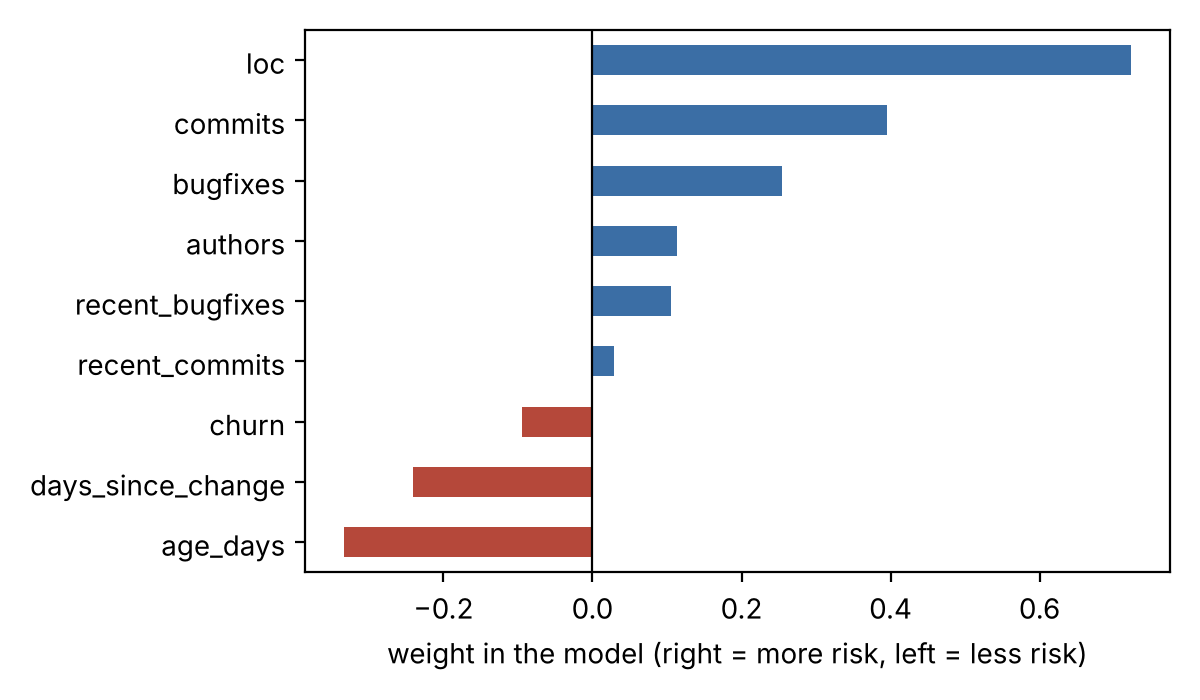
\includegraphics[width=0.75\textwidth]{feature_weights.png}}
{\fbox{Upload \texttt{results/feature\_weights.png} next to this file.}}
\caption{Weights of the features in the final model.}
\label{fig:weights}
\end{figure}

\subsection{Use on a live project and user feedback}
\label{sec:users}

The saved model can be applied to any git repository with one command:
\begin{verbatim}
python3 predict.py https://github.com/pallets/flask 5
\end{verbatim}
Flask is not part of the dataset. Run on 24~November 2026, the tool scored its
24 source files and ranked these five highest:

\begin{center}
\begin{tabular}{lrrrr}
\toprule
File & Risk & Lines & Commits & Authors \\
\midrule
\texttt{src/flask/app.py} & 0.93 & 1686 & 140 & 29 \\
\texttt{src/flask/cli.py} & 0.86 & 1126 & 67 & 18 \\
\texttt{src/flask/sansio/app.py} & 0.85 & 1014 & 20 & 6 \\
\texttt{src/flask/helpers.py} & 0.83 & 679 & 87 & 20 \\
\texttt{src/flask/sessions.py} & 0.70 & 385 & 33 & 8 \\
\bottomrule
\end{tabular}
\end{center}

To get feedback from users, the tool was run on a project each participant
knows well. They were shown the ten riskiest files and asked three questions.

\begin{center}
\begin{tabular}{p{2.6cm}p{3cm}p{2.6cm}p{2.6cm}p{2.6cm}}
\toprule
Participant & Project & Files of the 10 they also consider risky & A risky file that was missing? & Would use the list (1--5) \\
\midrule
\textbf{[fill in]} & \textbf{[fill in]} & \textbf{[fill in]} & \textbf{[fill in]} & \textbf{[fill in]} \\
\textbf{[fill in]} & \textbf{[fill in]} & \textbf{[fill in]} & \textbf{[fill in]} & \textbf{[fill in]} \\
\bottomrule
\end{tabular}
\end{center}

\todo{two or three sentences: what the participants agreed with, what
surprised them, and what they would want changed}

\section{Limitations}

\begin{itemize}
\item \textbf{Noisy labels.} Bug fixes are recognised by keywords in the commit
      message. Fixes that are worded differently are missed, and some commits
      with the word ``fix'' are not defects. This is a known problem of such
      data~\cite{herzig}.
\item \textbf{Size effect.} A large file is more likely to be touched by any
      commit, including a bug fix. Part of the model's success is this effect,
      as the comparison with the size rule shows.
\item \textbf{Renamed files.} A renamed file starts with an empty history, and
      a fix after a rename is not counted for the old name.
\item \textbf{Scope.} Only Python, only 12 open-source projects, and one
      cutoff date. The results may be different for other languages, for
      company projects, or for another year.
\item \textbf{Fixed threshold.} The 0.5 threshold gives very different
      precision in different projects (Table~\ref{tab:projects}).
\end{itemize}

\section{Future improvements}

\begin{itemize}
\item \textbf{Better labels}: use the issue tracker (commits linked to issues
      labelled ``bug'') instead of keywords.
\item \textbf{Predict bugs per line}, not per file, so that large files are
      not favoured automatically.
\item \textbf{Features from the code itself}, such as complexity or the number
      of imports, to add information that size and history do not have.
\item \textbf{More projects and languages}, and several cutoff dates per
      project to get more training data.
\item \textbf{A threshold per project}, for example ``flag the top 20\%'',
      instead of one fixed value.
\item \textbf{Integration in the workflow}: a bot that comments on a pull
      request when it touches a high-risk file.
\end{itemize}

\begin{thebibliography}{9}
\bibitem{ostrand} T. J. Ostrand, E. J. Weyuker, R. M. Bell. Predicting the
location and number of faults in large software systems. \emph{IEEE
Transactions on Software Engineering}, 31(4), 2005.
\bibitem{nagappan} N. Nagappan, T. Ball. Use of relative code churn measures
to predict system defect density. \emph{International Conference on Software
Engineering (ICSE)}, 2005.
\bibitem{moser} R. Moser, W. Pedrycz, G. Succi. A comparative analysis of the
efficiency of change metrics and static code attributes for defect prediction.
\emph{International Conference on Software Engineering (ICSE)}, 2008.
\bibitem{zimmermann} T. Zimmermann, N. Nagappan, H. Gall, E. Giger, B. Murphy.
Cross-project defect prediction: a large scale experiment on data vs. domain
vs. process. \emph{ESEC/FSE}, 2009.
\bibitem{zhang} F. Zhang, A. Mockus, I. Keivanloo, Y. Zou. Towards building a
universal defect prediction model. \emph{Working Conference on Mining Software
Repositories (MSR)}, 2014.
\bibitem{elemam} K. El Emam, S. Benlarbi, N. Goel, S. N. Rai. The confounding
effect of class size on the validity of object-oriented metrics. \emph{IEEE
Transactions on Software Engineering}, 27(7), 2001.
\bibitem{herzig} K. Herzig, S. Just, A. Zeller. It's not a bug, it's a
feature: how misclassification impacts bug prediction. \emph{International
Conference on Software Engineering (ICSE)}, 2013.
\bibitem{sklearn} F. Pedregosa et al. Scikit-learn: machine learning in
Python. \emph{Journal of Machine Learning Research}, 12, 2011.
\end{thebibliography}

\end{document}
